\section{Test Setup}
The Flink Cluster was built on a single physical host using virtualization and the SDN simulator
Mininet.

\subsection{Mininet}
Mininet is a software to simulate SDN environments on local machines. It  emulates physical hosts,
switches, links and routers on a Linux Kernel. \footnote{(2012). Introduction to Mininet ∙
mininet/mininet Wiki ∙ GitHub. Retrieved March 12, 2015, from
https://github.com/mininet/mininet/wiki/Introduction­to­Mininet} For topologies, either built-in or
shipped-with ones can be used or one can create custom topologies. Connected hosts are isolated from
each other and behave like real ones. For emulating switches, Mininet uses
Open-vSwitch\footnote{(2009). Open vSwitch. Retrieved March 12, 2015, from
httop://openvswitch.org/}, a virtual switch emulation software, controlled by OpenFlow.

With Mininet modeling all physical properties of a real SDN environment, ordinary network
diagnostics and manipulation software can be used. Also, Mininet is able to use a variety of SDN
controllers. The built-in one is based on POX but external ones can be connected by providing the
corresponding IP address and port number. For this work, we used the external controller option and
connected Mininet to an OpenDaylight controller.

Since the Mininet-network is emulated in an isolated environment, connected hosts do not have access
to the outer world, e.g. the Internet. To establish a connection, a Network Address Translation
Router (NAT) has to be connected. This is required to be able to communicate between cluster nodes
and the middleware.

\begin{figure}[h]
    \centering
    \begin{minipage}{0.5\textwidth}
        \centering
        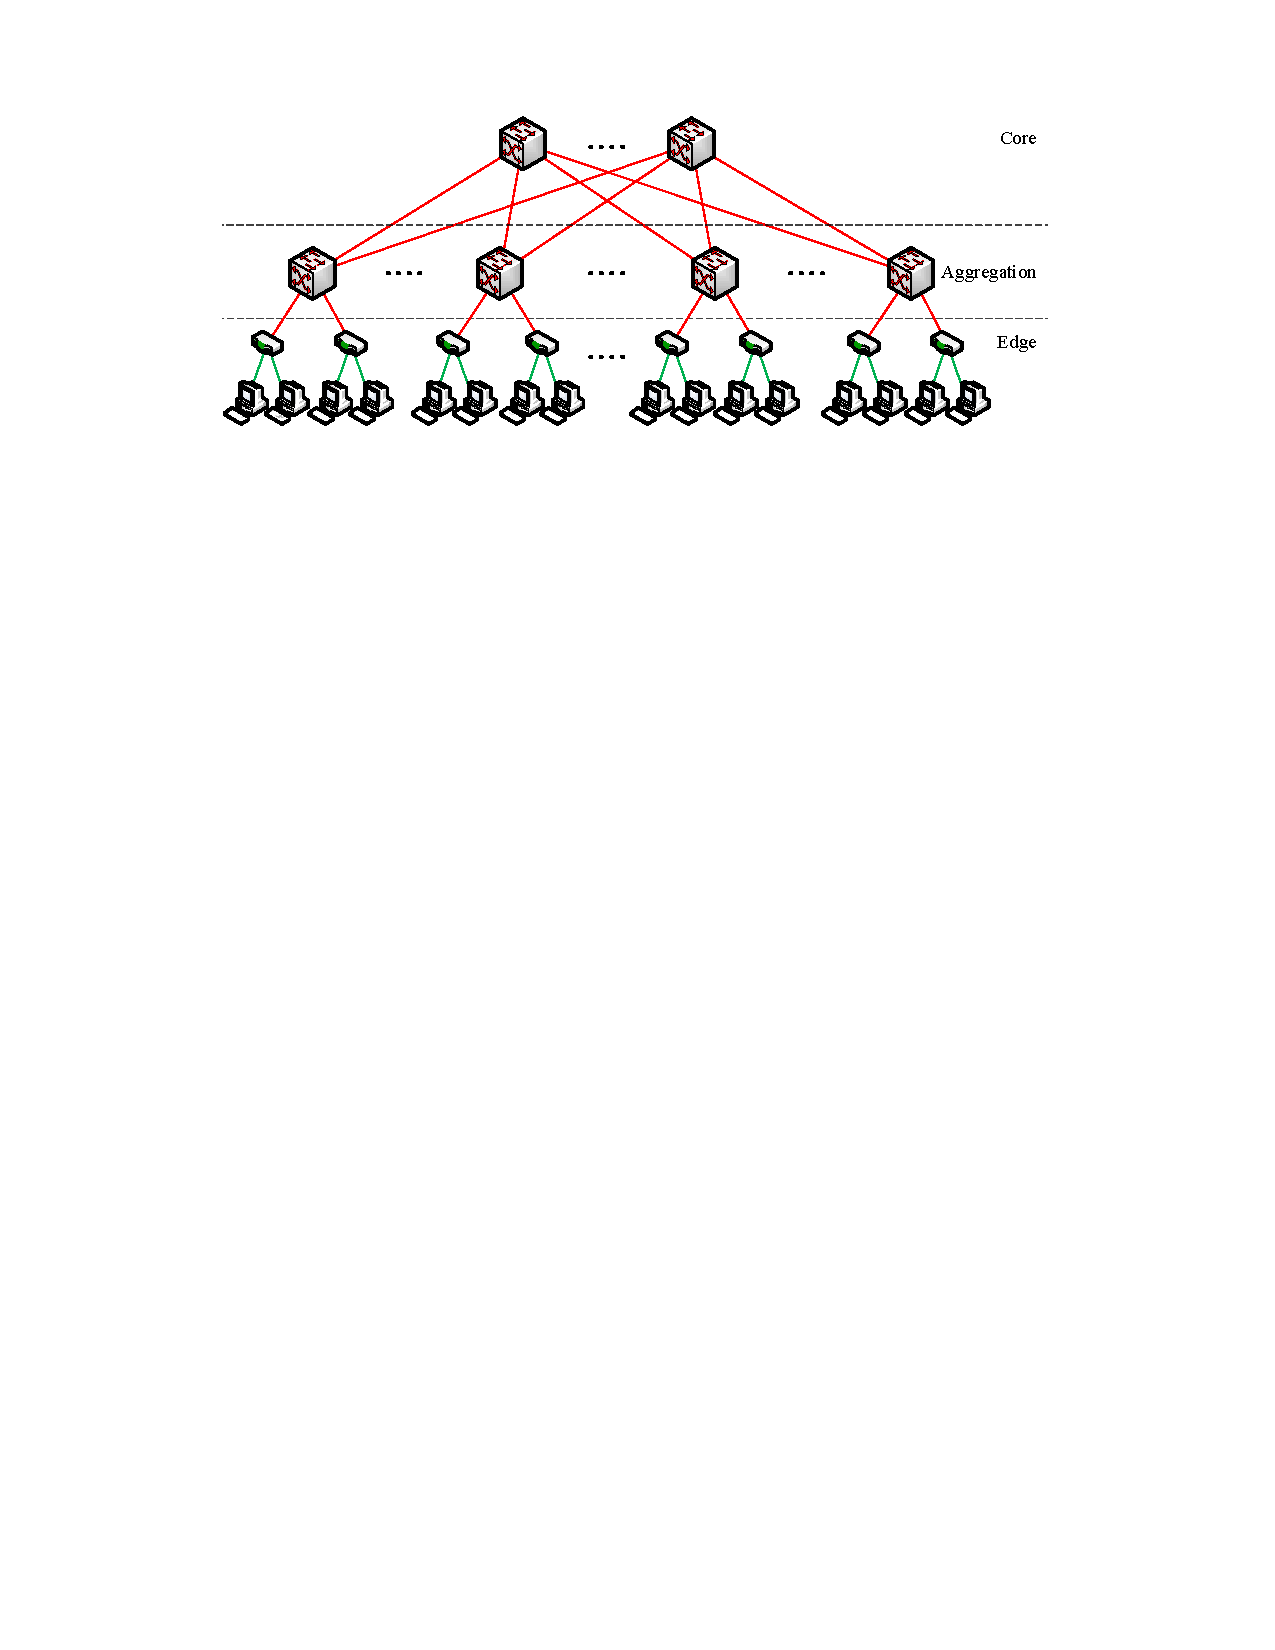
\includegraphics[width=1.0\linewidth]{graphics/typicalfattree.pdf}
        \captionof{figure}{Typical Fat-Tree setup \cite{datacenter}}
        \label{fig:typical_fattree}
    \end{minipage}%
    \begin{minipage}{0.5\textwidth}
        \centering
        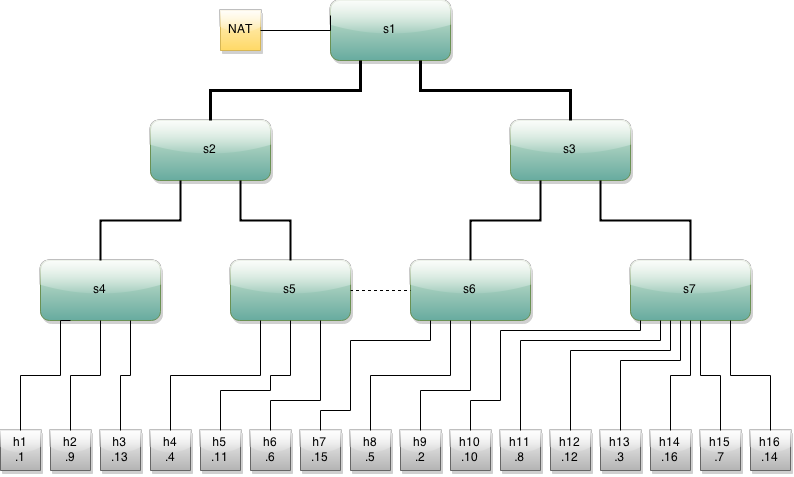
\includegraphics[width=1.0\linewidth]{graphics/mininetfattree.png}
        \captionof{figure}{Created Mininet topology}
        \label{fig:embedding}
    \end{minipage}
\end{figure}

\subsubsection{Typical Network Topology}
To evaluate the performance gain using the approach described in this paper, we need to create a
topology that resembles currently deployed network infrastructures at data centers as close as
possible. A common network structure is the so-called Fat Tree. \cite{datacenter} This topology
connects hosts and switches in a tree-like manner, with hosts on the lowest layer and switches in
the layers above.  Since link bandwidth increases with higher layers, the tree is called fat. A
sketch of this setup is depicted in the image below.

\subsection{System properties}
The test setup was built on a single physical host. Its physical properties are listed in the table
below.

\begin{table}[h]
    \centering
    \begin{tabular}{| l | l | }
        \hline
        \textbf{Property} & \textbf{Value} \\ \hline
        Operating &  System Windows 8.1 x64 \\ \hline
        CPU Intel & Core-i7 3720QM \\ \hline
        Memory & 8GB 1600MHz DDR3 \\ \hline
    \end{tabular}
    \caption{Physical host properties}
    \label{table:host_properties}
\end{table}

On top of the physical host, we implemented a virtualized testbed with the following properties.

\begin{table}[h]
    \centering
    \begin{tabular}{| l | l | }
        \hline
        \textbf{Property} & \textbf{Value} \\ \hline
        Virtualization software & VMWare Player 6.0.4 \\ \hline
        Operating System & Ubuntu 14.10 x64 \\ \hline
        Number of CPUs & 4 \\ \hline
        Memory & 5100MB \\ \hline
        Mininet & version 2.2.0rc2 \\ \hline
        Open vSwitch & version 2.1.3 \\ \hline
        OpenDaylight & version 0.2.2-SR2 \\ \hline
        Flink version & 0.7.0 incubating \\ \hline
    \end{tabular}
    \caption{Virtualized guest properties}
    \label{table:guest_properties}
\end{table}

Within the virtual guest, a mininet environment was built up with the topology described in the
mininet section of this paper. A Flink cluster was configured to handle every node as worker and use
128MB of heap per taskmanager. Further, a DoP of 5 was set. For all links, packet loss was set to 0\%
and delay to 2ms. Bandwidth was set to 5, 10 or 20MBit/s, depending on the link layer.

\subsection{Evaluation}
To evaluate the performance gain of our modified Flink setup, we compared job execution times of the
unmodified, native Flink application versus our SDN implementation. For KMeans, we used 5000
datapoints and a variable number of clusters and iterations. The results are shown in the following
table.

\begin{table}[h]
    \centering
    \begin{tabular}{| l | l | l | l | l | }
        \hline
        \textbf{No of Clusters} & \textbf{Iterations} & \textbf{Execution time}
            & \textbf{Execution time} & \textbf{Speedup in \%} \\
        & & \textbf{native in s} & \textbf{modified in s} & \\ \hline

        5 & 10 & 16.823 & 17.587 & -4.54 \\ \hline
        5 & 100 & 38.042 & 27.367 & 28.08 \\ \hline
        50 &10 &15.195 &9.689 &36.24 \\ \hline
        50 &100 &35.46 &19.979 &43.66 \\ \hline
        500 &10 &13.072 &9.166 &29.88 \\ \hline
        500 &100 &50.547 &24.378 &51.77 \\ \hline
    \end{tabular}
    \caption{Results of evaluation}
    \label{table:guest_properties}
\end{table}

As one can see, the implemented approach results in an overall speedup of the computation, merely
one configuration resulted in a performance decrease. It is remarkable that we gain up to 51.77\%
performance increase despite the fact that additional roundtrips are required for asking the
middleware for hosts to place the task on.
